\documentclass[11pt]{article}

\usepackage[margin=1.0in]{geometry}
\usepackage[utf8]{inputenc}
\usepackage[T1]{fontenc}
\usepackage{lmodern}
\usepackage{microtype}
\usepackage{amsmath,amssymb,amsthm}
\usepackage{booktabs}
\usepackage{graphicx}
\usepackage{xcolor}
\usepackage{enumitem}
\usepackage[
  colorlinks=true,
  linkcolor=blue!60!black,
  citecolor=blue!60!black,
  urlcolor=blue!60!black,
  pdftitle={Algebraic Gram Feasibility and Spectral Branch-and-Bound for the Hadamard Maximal Determinant Problem},
  pdfauthor={Bryan Sanchez},
  pdfsubject={Hadamard maximal determinant problem},
  pdfkeywords={Hadamard maximal determinant problem, D-optimal designs, Gram matrix realizability, Hasse-Minkowski theorem, Farkas lemma, Seidel switching, Cauchy interlacing}
]{hyperref}

\newtheorem{theorem}{Theorem}
\newtheorem{proposition}{Proposition}
\newtheorem{lemma}{Lemma}
\newtheorem{corollary}{Corollary}
\theoremstyle{remark}
\newtheorem{remark}{Remark}

\newcommand{\Z}{\mathbb{Z}}
\newcommand{\Q}{\mathbb{Q}}
\newcommand{\R}{\mathbb{R}}
\newcommand{\tr}{\operatorname{tr}}

\title{\textbf{Algebraic Gram Feasibility and Spectral Branch-and-Bound\\
for the Hadamard Maximal Determinant Problem}}

\author{%
  Bryan Sanchez\thanks{%
    Independent Researcher.
    E-mail: \texttt{bryansanchez.bas@gmail.com}.
    ORCID: \href{https://orcid.org/0009-0000-6080-5407}{0009-0000-6080-5407}.}
}

\date{November 26, 2026}

\begin{document}
\maketitle

\begin{abstract}
We develop an algebraic and spectral framework for upper bounds and obstructions in the Hadamard maximal determinant problem $D(n)=\max\{|\det M|:M\in\{\pm 1\}^{n\times n}\}$. The method combines exact rational $LDL^\top$ Hasse--Minkowski invariants, column-norm equations $x^\top G^{-1} x = 1$ for columns $x\in\{\pm 1\}^n$ of $M$ ($G = M M^\top$), and integer Farkas certificates with Seidel-gauge monotonicity, a positive-semidefinite trace Schur-complement inequality, and a closed-form Cauchy-interlaced Lagrange-dual branch-and-bound. First, for every $n \equiv 2 \pmod 4$, $n \ge 10$, the balanced two-block Gram matrix obtained from the extremal Ehlich--Wojtas matrix by flipping one off-diagonal $+2$ pair to $-2$ in each half is unrealizable as $M M^\top$. Second, we prove upper bounds strictly below the Ehlich--Wojtas bound $(2n-2)(n-2)^{(n-2)/2}$ for all six orders $n \equiv 2 \pmod 4$, $n \le 100$ with $2n-2$ not a sum of two squares ($n\in\{22,34,58,70,78,94\}$). Third, at $n = 34$, we prove $D(34) < 65 \cdot 32^{16}$, a full integer step below $66 \cdot 32^{16}$. Fourth, we exclude all $\{1,3,5\}$-supported Gram matrices at $n = 29$ with $\tr(G^2) < 25697$, vertex-disjoint off-diagonal $\pm 3, \pm 5$ pairs outside a normalized row, and $|\det M| \in [320,329)\cdot 7^{12}\cdot 2^{28}$, and every Gram matrix $G$ at $n = 33$ whose shifted matrix $G - J_{33}$ ($J_{33}$ the all-ones matrix) is block-diagonal of uniform cliques with off-diagonal entries in $\{-7,-3,1,5,9\}$ and $|\det M| \ge 441 \cdot 2^{74}$ ($9{,}220$ configurations with $G - J_{33} \succ 0$ above threshold).

\medskip
\noindent\textbf{MSC 2020:} 05B20, 15B34, 15A15, 62K05, 11E08.

\noindent\textbf{Keywords:} Hadamard maximal determinant problem; $D$-optimal designs; Gram matrix realizability; Hasse--Minkowski theorem; Farkas lemma; Seidel switching; Cauchy interlacing.
\end{abstract}

\section{Introduction}\label{sec:intro}

For each positive integer $n$, let
\[
  D(n) := \max \bigl\{ |\det M| : M \in \{\pm 1\}^{n \times n} \bigr\}
\]
denote the Hadamard maximal determinant of order $n$. Hadamard~\cite{hadamard1893} proved $D(n) \le n^{n/2}$, with equality if and only if $M M^\top = n I_n$ ($n \in \{1, 2\}$ or $n \equiv 0 \pmod 4$). For odd orders, Barba~\cite{barba1933} proved the general upper bound~\eqref{eq:barba} below; for $n \equiv 2 \pmod 4$, Ehlich~\cite{ehlich1964a} and Wojtas~\cite{wojtas1964} independently established the two-block upper bound~\eqref{eq:ew2}; and for $n \equiv 3 \pmod 4$, where Barba's bound is never attained for $n \ge 7$, Ehlich~\cite{ehlich1964b} obtained a sharper block-matrix bound. Classical structural theory, lower bounds, and small-order resolutions were developed by Cohn~\cite{cohn1963}, Moyssiadis and Kounias~\cite{moyssiadis1982}, Chadjipantelis, Kounias, and Moyssiadis~\cite{chadjipantelis1987}, Farmakis and Kounias~\cite{farmakis1987}, Neubauer and Radcliffe~\cite{neubauer1997}, Koukouvinos, Mitrouli, and Seberry~\cite{koukouvinos2000}, Orrick~\cite{orrick2005}, and Brent and Osborn~\cite{brent2013lower}. The two closed-form ceilings central to this work are Barba's bound~\eqref{eq:barba} and the Ehlich--Wojtas bound~\eqref{eq:ew2}:
\begin{align}
  D(n) &\le \sqrt{2n - 1}\,(n - 1)^{(n-1)/2}, && n \equiv 1 \pmod 4 \quad \text{(Barba~\cite{barba1933})}, \label{eq:barba}\\
  D(n) &\le (2n - 2)\,(n - 2)^{(n-2)/2}, && n \equiv 2 \pmod 4 \quad \text{(Ehlich--Wojtas~\cite{ehlich1964a,wojtas1964})}. \label{eq:ew2}
\end{align}
Throughout, we index rows and columns of $n \times n$ matrices by $\{1, \dots, n\}$. Any realizable matrix $M \in \{\pm 1\}^{n \times n}$ induces a symmetric positive-semidefinite integer Gram matrix $G = M M^\top$ with diagonal $G_{ii} = n$ and parity-constrained off-diagonal entries $G_{ij} \equiv n \pmod 2$. Writing $\mathbf{r} = M \mathbf{1}$ for the row-sum vector and $A = \frac{1}{2}(M + J) \in \{0, 1\}^{n \times n}$, the identity $G_{ij} = 4(A A^\top)_{ij} - n - r_i - r_j$ forces
\begin{equation}\label{eq:div4}
  n + r_i + r_j + G_{ij} \equiv 0 \pmod 4 \qquad (1 \le i, j \le n).
\end{equation}

Equality in Barba's bound~\eqref{eq:barba} requires $2n - 1$ to be an odd perfect square; equality in the Ehlich--Wojtas bound~\eqref{eq:ew2} requires $2n - 2$ to be a sum of two integer squares (equivalently, every prime $p \equiv 3 \pmod 4$ dividing $2n - 2$ must occur to an even exponent). As documented in the survey of Browne, Egan, Hegarty, and \'O~Cath\'ain~\cite{browne2021survey}, the exceptional orders $n \equiv 2 \pmod 4$ with $n \le 100$ for which $2n - 2$ is not a sum of two squares are
\[
  n \in \{22, 34, 58, 70, 78, 94\}.
\]
Order $n = 22$ was resolved ($D(22) = 40 \cdot 20^{10} < 42 \cdot 20^{10}$) by Chasiotis, Kounias, and Farmakis~\cite{chasiotis2018,chasiotis2019corr}, leaving $n = 34$ as the smallest open exceptional order in the $2 \pmod 4$ class. In the $1 \pmod 4$ class, the smallest open orders are $n = 29$, where the unpublished preprint of Brent, Orrick, Osborn, and Zimmermann~\cite{brent2012maximal} reports $320 \cdot 7^{12} \cdot 2^{28} \le D(29) < 329 \cdot 7^{12} \cdot 2^{28}$ and notes that if $7^{13}$ divides $D(29)/2^{28}$ then $D(29) = 322 \cdot 7^{12} \cdot 2^{28}$, and $n = 33$, where Solomon's lower bound stands at $441 \cdot 2^{74}$ against Barba's ceiling $\lfloor\sqrt{65}\cdot 2^{80}\rfloor \approx 515.98 \cdot 2^{74}$~\cite{orrick2003,orrick2007,brent2012maxdet}.

Direct combinatorial search over $M M^\top = G$ scales poorly even at $n = 29$ because the $O(n^2)$ quadratic inner-product equations introduce heavy symmetry and weak local propagation. In this paper we pair exact algebraic realizability obstructions (Section~\ref{sec:algebraic}) with sharp spectral relaxations and branch-and-bound to obtain four main results. In Section~\ref{sec:k2k2} we give a short elementary proof that for every $k \ge 2$ ($n = 4k + 2 \ge 10$, $h = 2k + 1$), the leading balanced $C = 0$ perturbation $(h, h)\, K_2 \oplus K_2$ is never realizable as $M M^\top$ over $\{\pm 1\}^{n \times n}$ (Theorem~\ref{thm:k2k2}). In Section~\ref{sec:spectral} we combine Seidel-gauge monotonicity, a KKT-certified capped-spectrum bound (Proposition~\ref{prop:capped_seidel}), and an exact positive-semidefinite (PSD) trace Schur-complement inequality (Proposition~\ref{prop:psd_trace}) to prove unconditional upper bounds strictly below the Ehlich--Wojtas bound for all six exceptional orders $n \in \{22, 34, 58, 70, 78, 94\}$ (Theorem~\ref{thm:r2_all}). In Section~\ref{sec:d34} we introduce a closed-form 15-dual Cauchy-interlaced Lagrange-dual branch-and-bound (Proposition~\ref{prop:tangent_dual}) that breaks past the $2$-moment spectral barrier ($65.453 \cdot 32^{16}$) at $n = 34$ and eliminates all remaining $C = 0$ and $C \ne 0$ candidates, establishing $D(34) < 65 \cdot 32^{16} = 65 \cdot 2^{80}$ (Theorem~\ref{thm:d34}). Finally, in Section~\ref{sec:r1} we apply our exact algebraic filters to the $n \equiv 1 \pmod 4$ class, eliminating all $11$ residual low-trace spread-placement candidates at $n = 29$ in $[320, 329) \cdot 7^{12} \cdot 2^{28}$ (with compact integer Farkas certificates for both candidates at $322 \cdot 7^{12} \cdot 2^{28}$) and excluding every Gram matrix $G = 32 I_{33} + J_{33} + 4E$ at $n = 33$ whose shifted matrix $G - J_{33}$ is block-diagonal with off-diagonal entries in $\{-7, -3, 1, 5, 9\}$ and $|\det M| \ge 441 \cdot 2^{74}$ ($9{,}220$ complete $G - J_{33} \succ 0$ configurations above threshold, $3{,}764$ for clique weights $w_i \in \{\pm 1\}$, enumerated via exact integer branch-and-bound; Theorem~\ref{thm:r1_close}).

\section{Exact Algebraic Realizability Obstructions}\label{sec:algebraic}

Filtering candidate Gram matrices prior to explicit $\{\pm 1\}$ decomposition is a classical strategy in $D$-optimal design theory and maximal determinant proofs, going back to Moyssiadis and Kounias~\cite{moyssiadis1982}, Chadjipantelis, Kounias, and Moyssiadis~\cite{chadjipantelis1987}, Farmakis and Kounias~\cite{farmakis1987}, Neubauer and Radcliffe~\cite{neubauer1997}, Orrick~\cite{orrick2005}, and Brent, Orrick, Osborn, and Zimmermann~\cite{brent2012maximal}. We organize these necessary conditions into four exact rational and arbitrary-precision integer tests for a symmetric positive-definite integer Gram candidate $G \in \Z^{n \times n}$ with $G_{ii} = n$.

\begin{enumerate}[leftmargin=*,topsep=3pt,itemsep=2pt]
\item \textbf{Exact perfect-square determinant.} Since $\det G = (\det M)^2$, $\det G$ must be an exact integer square. We compute $\det G$ via fraction-free Bareiss elimination (or block Schur reduction) over exact integers and test $\lfloor\sqrt{\det G}\rfloor^2 = \det G$.
\item \textbf{Hasse--Minkowski rational congruence.} If $G = M M^\top$ for $M \in \mathrm{GL}_n(\Q)$, then $G$ is rationally congruent to $I_n$~\cite{serre1973}. Exact rational $LDL^\top$ diagonalization produces positive rational pivots $d_1, \dots, d_n \in \Q_{>0}$. Writing $a_i := p_i q_i \in \Z_{>0}$ for $d_i = p_i / q_i$ (preserving square classes in $\Q^\times / (\Q^\times)^2$), the Hasse invariant at every prime $p \mid 2\det G$ must satisfy
\begin{equation}\label{eq:hasse}
  c_p(G) := \prod_{1 \le i < j \le n} (a_i, a_j)_p = +1,
\end{equation}
where $(a, b)_p \in \{\pm 1\}$ is the Hilbert symbol over $\Q_p$~\cite[Ch.~III--IV]{serre1973}. Any prime $p$ with $c_p(G) = -1$ proves $G \not\simeq_\Q I_n$, hence $G$ is unrealizable over $\Z$.
\item \textbf{Exact column-norm equation $x^\top G^{-1} x = 1$.} Since $G \succ 0$ is invertible, $M M^\top = G$ is equivalent to $M^\top G^{-1} M = I_n$. In particular, every column $x \in \{\pm 1\}^n$ of $M$ must satisfy
\begin{equation}\label{eq:colnorm}
  x^\top G^{-1} x = 1.
\end{equation}
Whenever the automorphism group of $G$ partitions $\{1, \dots, n\}$ into symmetry orbits $g_1, \dots, g_q$ (for example, uniform cliques and singletons), the quadratic form $x^\top G^{-1} x$ depends only on the orbit sums $s_a = \sum_{i \in g_a} x_i$ (together with any small active subgraph coordinates). Exact rational enumeration over all parity-valid orbit sums immediately detects: (a) \emph{zero-solution} obstructions, and (b) \emph{forced-identity} obstructions where every solution forces $x_i = x_j$ (or $x_i = -x_j$) on some pair $(i, j)$, implying $G_{ij} = \pm n$, contradicting $|G_{ij}| < n$.
\item \textbf{Exact integer Farkas certificates.} Suppose $t$ orbit-sum column types $j \in \{1, \dots, t\}$ satisfy~\eqref{eq:colnorm}, with unknown non-negative integer multiplicities $n_1, \dots, n_t \in \Z_{\ge 0}$ in $M$. Summing across all $n$ columns yields an exact linear moment system $A \mathbf{n} = \mathbf{b}$:
\[
  \sum_{j=1}^t n_j = n, \qquad
  \sum_{j=1}^t n_j s_{a,j} = \mathbf{1}_{g_a}^\top \mathbf{r}, \qquad
  \sum_{j=1}^t n_j s_{a,j} s_{b,j} = \mathbf{1}_{g_a}^\top G \mathbf{1}_{g_b} \quad (1 \le a \le b \le q).
\]
To certify infeasibility independently of any linear-programming solver, we exhibit an explicit integer vector $y \in \Z^m$ and verify in exact integer arithmetic that
\begin{equation}\label{eq:farkas}
  y^\top A_j \ge 0 \quad \forall j \in \{1, \dots, t\}, \qquad\text{and}\qquad y^\top \mathbf{b} < 0.
\end{equation}
By Farkas's lemma,~\eqref{eq:farkas} proves that no non-negative real (a fortiori integer) multiplicity vector $\mathbf{n}$ exists.
\end{enumerate}

\section{Infinite-Family Obstruction for \texorpdfstring{$n \equiv 2 \pmod 4$}{n = 2 (mod 4)}}\label{sec:k2k2}

For $n \equiv 2 \pmod 4$, write $n = 4k + 2$ ($k \ge 2$), $h = n/2 = 2k + 1$, and $m = n - 2 = 4k$. Partitioning the rows of $M \in \{\pm 1\}^{n \times n}$ by pairwise inner-product residue modulo $4$ (equivalently, by row-sum residue modulo $4$ after normalizing a fixed column) places the Gram matrix in the Ehlich--Wojtas two-block form~\cite{ehlich1964a,wojtas1964}
\begin{equation}\label{eq:twoblock}
  G = \begin{pmatrix} B_1 & C \\ C^\top & B_2 \end{pmatrix}, \qquad s_1 + s_2 = n, \; s_1 \le h,
\end{equation}
where $(B_\ell)_{ij} \equiv 2 \pmod 4$ for $i \ne j$ and $C_{ij} \equiv 0 \pmod 4$.

At the balanced split $s_1 = s_2 = h$ with $C = 0$, the extremal Ehlich--Wojtas Gram matrix has $B_1 = B_2 = m I_h + 2 J_h$ (denoted $\emptyset \oplus \emptyset$), whose determinant is $(2n - 2)^2 m^{n-2}$. Whenever $2n - 2 = 8k + 2$ is not a sum of two squares, $\emptyset \oplus \emptyset$ fails Hasse--Minkowski. Flipping a single off-diagonal pair in each block from $+2$ to $-2$ produces the leading balanced $C = 0$ perturbation $B = m I_h + 2 J_h - 4 E_{12}$, where $(E_{12})_{12} = (E_{12})_{21} = 1$ and all other entries vanish. Its block Gram matrix $G = B \oplus B$, denoted $(h, h)\, K_2 \oplus K_2$, splits $\R^{2k+1}$ into the $1$-dimensional span of $e_1 - e_2$ (eigenvalue $4k + 4$), the $(2k-2)$-dimensional orthocomplement of $\mathbf{1}$ inside $\{3, \dots, 2k+1\}$ (eigenvalue $4k$), and the $2$-dimensional span of $\{e_1 + e_2, \sum_{j=3}^{2k+1} e_j\}$, on which the quotient matrix is
\[
  \begin{pmatrix} 4k & 2(2k-1) \\ 4 & 8k - 2 \end{pmatrix},
  \qquad \det = 4k(8k - 2) - 8(2k - 1) = 8(4k^2 - 3k + 1).
\]
Hence $\det B = 8(4k^2 - 3k + 1)(4k + 4)(4k)^{2k-2} = \frac{2(k + 1)(4k^2 - 3k + 1)}{k^2}\, m^{h-1}$, so $\det(B \oplus B) = (\det B)^2$ is always a perfect square. For any direct sum of two identical symmetric rational blocks, $c_p(B \oplus B) = (-1, \det B)_p$ (off-diagonal cross-pairs cancel in squares while diagonal pairs $(d_i, d_i)_p = (-1, d_i)_p$ multiply to $(-1, \det B)_p$). Thus $(h, h)\, K_2 \oplus K_2$ fails Hasse--Minkowski whenever $2(k + 1)(4k^2 - 3k + 1)$ carries an odd-exponent prime $\equiv 3 \pmod 4$ (as occurs at $n \in \{22, 58, 70, 78, 94\}$), but passes Hasse--Minkowski whenever that product is a sum of two squares, notably at $n = 34$ ($k = 8$, where $2 \cdot 9 \cdot 233 = 2 \cdot 3^2 \cdot 233$ with $233 \equiv 1 \pmod 4$) and $k \in \{9, 12, \dots\}$. Theorem~\ref{thm:k2k2} rules out $(h, h)\, K_2 \oplus K_2$ uniformly for all $k \ge 2$ via a short elementary proof.

\begin{theorem}[Infinite-family obstruction for $(h, h)\, K_2 \oplus K_2$]\label{thm:k2k2}
For every integer $k \ge 2$ (that is, every $n = 4k + 2 \ge 10$, $h = 2k + 1$), the two-block Gram matrix $G = B \oplus B$ with $B = (n - 2) I_h + 2 J_h - 4 E_{12}$ has no realization $G = M M^\top$ with $M \in \{\pm 1\}^{n \times n}$.
\end{theorem}

\begin{proof}
Write $B = 2 A + 2 \mathbf{1}\mathbf{1}^\top$, where $A = \operatorname{diag}\!\bigl(\begin{pmatrix} 2k & -2 \\ -2 & 2k \end{pmatrix}, 2k I_{2k-1}\bigr)$. The eigenvalues of $A$ on the first two coordinates are $2(k - 1)$ (on $e_1 + e_2$) and $2(k + 1)$ (on $e_1 - e_2$), and $2k$ on the remaining $2k - 1$ coordinates. Let
\[
  D := 1 + \mathbf{1}^\top A^{-1} \mathbf{1}
  = 1 + \frac{1}{k - 1} + \frac{2k - 1}{2k}
  = \frac{4k^2 - 3k + 1}{2k(k - 1)}.
\]
By the Sherman--Morrison formula, $B^{-1} = \frac{1}{2}\bigl(A^{-1} - D^{-1} A^{-1}\mathbf{1}\mathbf{1}^\top A^{-1}\bigr)$.

Consider any column $x = (y_1, y_2) \in \{\pm 1\}^h \times \{\pm 1\}^h$ of $M$, which must satisfy $y_1^\top B^{-1} y_1 + y_2^\top B^{-1} y_2 = 1$. For each half $y_i \in \{\pm 1\}^h$, let $s_i := \sum_{j=3}^{2k+1} y_{i,j} \in \Z$ (an odd integer), and classify $y_i$ as $\mathrm{same}$ if $y_{i,1} = y_{i,2} = \epsilon_i \in \{\pm 1\}$ or $\mathrm{opp}$ if $y_{i,1} = -y_{i,2}$. Direct substitution gives
\begin{align*}
  2 y_i^\top B^{-1} y_i - 1
  &= \begin{cases}
    \displaystyle \left(\frac{1}{k - 1} + \frac{2k - 1}{2k} - 1\right) - \frac{1}{D}\left(\frac{\epsilon_i}{k - 1} + \frac{s_i}{2k}\right)^2 & (\mathrm{same}), \\[10pt]
    \displaystyle \left(\frac{1}{k + 1} + \frac{2k - 1}{2k} - 1\right) - \frac{1}{D}\left(\frac{s_i}{2k}\right)^2 & (\mathrm{opp}).
  \end{cases}
\end{align*}
The column equation $y_1^\top B^{-1} y_1 + y_2^\top B^{-1} y_2 = 1$ is equivalent to $(2 y_1^\top B^{-1} y_1 - 1) + (2 y_2^\top B^{-1} y_2 - 1) = 0$. Clearing denominators produces two cases whenever at least one half is $\mathrm{opp}$:

\begin{itemize}[leftmargin=*,topsep=3pt,itemsep=2pt]
\item \textbf{Case 1 ($\mathrm{opp} + \mathrm{opp}$).} Simplifying gives
\[
  (k + 1)(s_1^2 + s_2^2) = 2(4k^2 - 3k + 1).
\]
Since $2(4k^2 - 3k + 1) = (k + 1)(8k - 14) + 16$, divisibility by $k + 1$ forces $(k + 1) \mid 16$. As $k \ge 2$, we must have $k \in \{3, 7, 15\}$, giving $s_1^2 + s_2^2 \in \{14, 44, 107\}$. None of $14 = 2 \cdot 7$, $44 = 2^2 \cdot 11$, or $107$ (prime $\equiv 3 \pmod 4$) is a sum of two integer squares.

\item \textbf{Case 2 ($\mathrm{same} + \mathrm{opp}$, or symmetrically $\mathrm{opp} + \mathrm{same}$).} Set $X_1 := 2k \epsilon_1 + (k - 1) s_1 \in \Z$, so $\frac{\epsilon_1}{k - 1} + \frac{s_1}{2k} = \frac{X_1}{2k(k - 1)}$. Clearing denominators yields
\[
  (k + 1)\bigl(X_1^2 + (k - 1)^2 s_2^2\bigr) = 2(k^2 + 1)(4k^2 - 3k + 1).
\]
Polynomial division gives $2(k^2 + 1)(4k^2 - 3k + 1) \equiv 32 \pmod{k + 1}$, so $(k + 1) \mid 32$ and $k \in \{3, 7, 15, 31\}$. The corresponding right-hand quotients are
\begin{align*}
  k = 3:  &\quad 140 = 2^2 \cdot 5 \cdot 7, &
  k = 7:  &\quad 2200 = 2^3 \cdot 5^2 \cdot 11, \\
  k = 15: &\quad 24182 = 2 \cdot 113 \cdot 107, &
  k = 31: &\quad 225589 = 7 \cdot 13 \cdot 37 \cdot 67,
\end{align*}
each of which carries a prime $\equiv 3 \pmod 4$ ($7, 11, 107, 7$ respectively) to an odd exponent, so none is a sum of two integer squares.
\end{itemize}

Therefore every column $x = (y_1, y_2)$ of $M$ must be $\mathrm{same} + \mathrm{same}$, forcing $y_{1,1} = y_{1,2}$ in every column. This implies $G_{1,2} = \sum_{j=1}^n M_{1j} M_{2j} = n$, contradicting $G_{1,2} = -2$.
\end{proof}

\section{Spectral Bounds for Exceptional Orders \texorpdfstring{$n \equiv 2 \pmod 4$}{n = 2 (mod 4)}}\label{sec:spectral}

Write any $s \times s$ diagonal block $B$ in~\eqref{eq:twoblock} as $B = n I_s + 2 S$, where $S$ is a symmetric integer matrix with zero diagonal and odd off-diagonal entries $S_{ij} \in \{\pm 1, \pm 3, \pm 5, \dots\}$. Denote by $m_6(B)$ the number of off-diagonal pairs $\{i, j\}$ with $|B_{ij}| \ge 6$ (equivalently $|S_{ij}| \ge 3$). When $m_6(B) = 0$, $S$ is a \emph{Seidel matrix} (all off-diagonal entries $\pm 1$), and conjugating $S \mapsto D S D$ by a diagonal sign matrix $D \in \{\pm 1\}^{s \times s}$ is Seidel switching~\cite{brouwer2012}, which preserves the spectrum of $B$ and corresponds to row negations of $M$.

\begin{proposition}[Seidel-gauge monotonicity and capped-spectrum upper bound]\label{prop:capped_seidel}
Let $B = n I_s + 2 S \succ 0$ ($s \ge 3$) with $\tr(S) = 0$ and $\tr(S^2) = s(s - 1) + \Delta_S$ ($\Delta_S \ge 0$).
\begin{enumerate}[leftmargin=*,topsep=2pt,itemsep=1pt]
\item \emph{(Seidel-gauge monotonicity.)} There exists a diagonal sign matrix $D \in \{\pm 1\}^{s \times s}$ such that a top unit eigenvector $v$ of $\widetilde{S} = D S D$ satisfies $v_i \ge 0$ for all $i \in \{1, \dots, s\}$. If $m_6(B) = 0$ and $H$ is the graph of $-1$ entries of $\widetilde{S}$, then for every subgraph $H' \subseteq H$,
\[
  \lambda_{\max}(S) = v^\top \widetilde{S} v \le v^\top S(H') v \le \lambda_{\max}\bigl(S(H')\bigr),
\]
where $S(H')$ has $-1$ on edges of $H'$ and $+1$ on non-edges. More generally, for any $m_6 \ge 1$ with $|S_{ij}| = 3$ on an edge set $E_6$ ($|E_6| = m_6$) and $|S_{ij}| = 1$ elsewhere, replacing every negative entry of $\widetilde{S}$ by $|\widetilde{S}_{ij}|$ gives $\lambda_{\max}(S) \le \lambda_{\max}(S_{E_6}^{\emptyset})$, where $S_{E_6}^{\emptyset}$ has $+3$ on $E_6$ and $+1$ on all other off-diagonals.
\item \emph{(Capped-spectrum maximum.)} For any upper cap $\mu_{\mathrm{cap}} > 0$ satisfying $\lambda_{\max}(S) \le \mu_{\mathrm{cap}}$, we have $\det B \le \Phi_{\max}(n, s, \Delta_S; \mu_{\mathrm{cap}})$, where
\begin{multline*}
  \Phi_{\max}(n, s, \Delta_S; \mu_{\mathrm{cap}})
  := \max \Bigl\{ \prod_{j=1}^s (n + 2\mu_j) : \sum_{j=1}^s \mu_j = 0, \\
  \sum_{j=1}^s \mu_j^2 = s(s - 1) + \Delta_S,\; -\frac{n}{2} < \mu_j \le \mu_{\mathrm{cap}} \Bigr\}.
\end{multline*}
Moreover, $\Phi_{\max}$ is monotonically non-decreasing in $\mu_{\mathrm{cap}}$, and every global maximizer has the form $(\mu_{\mathrm{cap}}^{(r)}, a^{(s - r - 1)}, b)$ for some integer $r \ge 0$ and $a \le b \le \mu_{\mathrm{cap}}$ (or $a = b$ if the remaining variance vanishes). In particular, whenever the global maximum over $r \ge 0$ is attained at $r = 1$ with $b \le \mu_{\mathrm{cap}}$,
\begin{equation}\label{eq:seidel_var}
  \det B \le (n + 2\mu_{\mathrm{cap}})\,(n + 2a)^{s-2}\,(n + 2b),
\end{equation}
where $\bar{\mu} = -\mu_{\mathrm{cap}}/(s-1)$, $V_2 = s(s-1) + \Delta_S - \mu_{\mathrm{cap}}^2 - \mu_{\mathrm{cap}}^2/(s-1)$, $x = \sqrt{V_2 / ((s-1)(s-2))}$, $a = \bar{\mu} - x$, and $b = \bar{\mu} + (s-2)x$.
\end{enumerate}
\end{proposition}

\begin{proof}
For Part~(1), let $w$ be any top unit eigenvector of $S$ and define $D = \operatorname{diag}(d_1, \dots, d_s)$ by $d_i = +1$ if $w_i \ge 0$ and $d_i = -1$ if $w_i < 0$; then $v = D w$ is a top unit eigenvector of $\widetilde{S} = D S D$ with $v_i = |w_i| \ge 0$ for all $i$. Flipping any negative entry of $\widetilde{S}$ to its absolute value increases $\widetilde{S}_{ij}$ while $v_i v_j \ge 0$, proving both inequalities.

For Part~(2), $\det B \le \Phi_{\max}$ holds directly from $\lambda_{\max}(S) \le \mu_{\mathrm{cap}}$, and monotonicity in $\mu_{\mathrm{cap}}$ follows from nested feasible sets. Extending the objective $\prod_{j=1}^s (n + 2\mu_j)$ to the compact closure $-n/2 \le \mu_j \le \mu_{\mathrm{cap}}$, any boundary point with $\mu_j = -n/2$ has objective value $0$, so every positive global maximizer $\mu^*$ lies in $(-n/2, \mu_{\mathrm{cap}}]^s$. At $\mu^*$, if all strictly interior coordinates ($\mu_j^* < \mu_{\mathrm{cap}}$) are equal, we are in the $a = b$ boundary case; otherwise, at least two interior coordinates are distinct, so the linear independence constraint qualification (LICQ) holds for the linear and quadratic equality constraints, and the KKT conditions yield Lagrange multipliers $\alpha, \gamma \in \R$ and $\nu_j \ge 0$ with $\nu_j(\mu_j^* - \mu_{\mathrm{cap}}) = 0$ and
\[
  \frac{2}{n + 2\mu_j^*} = 2\alpha \mu_j^* + \gamma + \nu_j \qquad (j = 1, \dots, s).
\]
Every strictly interior coordinate ($\mu_j^* < \mu_{\mathrm{cap}}$, so $\nu_j = 0$) satisfies the quadratic equation $p(\mu) := (n + 2\mu)(\alpha \mu + \gamma/2) - 1 = 0$, which has at most two real roots $a < b < \mu_{\mathrm{cap}}$. When two distinct roots exist, necessarily $\alpha \ne 0$, and since $p(-n/2) = -1 < 0$ while $a, b > -n/2$, we must have $\alpha < 0$; equivalently, $f(\mu) := \ln(n + 2\mu) - \alpha \mu^2 - \gamma\mu$ has strictly concave $\ln(n+2\mu)$ and two critical points $a < b$, forcing $f''(a) < 0$ and $f''(b) > 0$. If the upper root $b$ occurred with multiplicity at least $2$ alongside a distinct interior coordinate $a$, then LICQ holds on the constant-sum, constant-variance manifold for the triple $(a, b, b)$, and the first-order tangent direction $(0, +1, -1)$ gives second-order Lagrangian variation $2 f''(b) > 0$, contradicting the second-order necessary condition for maximality. Hence $b$ has multiplicity at most $1$, and every maximizer has the stated $(r, s-r-1, 1)$ structure; $r = 1$ gives~\eqref{eq:seidel_var}.
\end{proof}

\begin{proposition}[Exact PSD trace Schur-complement lower bound]\label{prop:psd_trace}
Let $G = \begin{pmatrix} B_1 & C \\ C^\top & B_2 \end{pmatrix} \succ 0$, where $B_1$ has eigenvalues $\lambda_1 \ge \lambda_2 \ge \dots > 0$ with top unit eigenvector $v_1$, and $B_2$ has eigenvalues $\mu_1 \ge \mu_2 \ge \dots > 0$ with top unit eigenvector $v_2$. Suppose $C$ has $k \ge 1$ nonzero entries and Frobenius norm squared $F = \|C\|_F^2$. Setting $a_i := \min(1, k \|v_i\|_\infty^2)$ for $i \in \{1, 2\}$, we have
\begin{equation}\label{eq:psd_trace}
  \det G \le \det(B_1)\det(B_2)\,\exp\bigl(-\max\{T_{\mathrm{mode}}(k, F),\, T_{\mathrm{crude}}(F)\}\bigr),
\end{equation}
where $T_{\mathrm{crude}}(F) := F / (\lambda_1 \mu_1)$ and
\[
  T_{\mathrm{mode}}(k, F) := \frac{F}{\lambda_2 \mu_2}
  - \left(\frac{1}{\lambda_2} - \frac{1}{\lambda_1}\right)\frac{a_1 F}{\mu_2}
  - \left(\frac{1}{\mu_2} - \frac{1}{\mu_1}\right)\frac{a_2 F}{\lambda_2}.
\]
\end{proposition}

\begin{proof}
By the Schur complement identity, $\det G = \det(B_1)\det(B_2)\det(I - X)$, where
\[
  X := B_2^{-1/2} C^\top B_1^{-1} C B_2^{-1/2}
\]
satisfies $0 \preceq X \prec I$. Since $1 - \sigma \le e^{-\sigma}$ for $\sigma \in [0, 1)$, $\det(I - X) \le \exp(-\tr X)$. Clearly $\tr X \ge \|C\|_F^2 / (\lambda_1 \mu_1) = T_{\mathrm{crude}}(F)$. For the sharpened bound, spectral decomposition gives
\begin{align*}
  B_1^{-1} &\succeq \frac{1}{\lambda_2} I - \left(\frac{1}{\lambda_2} - \frac{1}{\lambda_1}\right) v_1 v_1^\top, \\
  B_2^{-1} &\succeq \frac{1}{\mu_2} I - \left(\frac{1}{\mu_2} - \frac{1}{\mu_1}\right) v_2 v_2^\top.
\end{align*}
Substituting into $\tr(B_2^{-1} C^\top B_1^{-1} C)$ and dropping the non-negative rank-one cross term $+\bigl(\frac{1}{\lambda_2} - \frac{1}{\lambda_1}\bigr)\bigl(\frac{1}{\mu_2} - \frac{1}{\mu_1}\bigr)(v_1^\top C v_2)^2 \ge 0$ gives
\[
  \tr X \ge \frac{F}{\lambda_2 \mu_2}
  - \left(\frac{1}{\lambda_2} - \frac{1}{\lambda_1}\right)\frac{\|C^\top v_1\|_2^2}{\mu_2}
  - \left(\frac{1}{\mu_2} - \frac{1}{\mu_1}\right)\frac{\|C v_2\|_2^2}{\lambda_2}.
\]
For each column $j$ of $C$ with $k_j \le k$ nonzero entries, Cauchy--Schwarz gives $(\sum_i C_{ij} v_{1,i})^2 \le (\sum_i C_{ij}^2)\min(1, k_j \|v_1\|_\infty^2) \le a_1 \sum_i C_{ij}^2$, so $\|C^\top v_1\|_2^2 \le a_1 F$ and symmetrically $\|C v_2\|_2^2 \le a_2 F$.
\end{proof}

\begin{theorem}[Upper bounds strictly below the Ehlich--Wojtas bound for $n \le 100$]\label{thm:r2_all}
For every exceptional order $n \in \{22, 34, 58, 70, 78, 94\}$, the maximal determinant satisfies $D(n) < c_n^{(2)} \cdot (n - 2)^{(n-2)/2}$ strictly below the Ehlich--Wojtas bound $(2n - 2)(n - 2)^{(n-2)/2}$, with
\begin{align*}
  c_{22}^{(2)} &= 41.386, & c_{34}^{(2)} &= 65.453, & c_{58}^{(2)} &= 113.604, \\
  c_{70}^{(2)} &= 137.663, & c_{78}^{(2)} &= 153.697, & c_{94}^{(2)} &= 185.748.
\end{align*}
\end{theorem}

\begin{proof}
For each $n$, let $h = n/2$, $m = n - 2$, and set $c_n = c_n^{(2)}$. Every $M \in \{\pm 1\}^{n \times n}$ has a two-block Gram matrix~\eqref{eq:twoblock} with $s_1 \le h$. By Fischer's inequality $\det G \le \det B_1 \det B_2$:
\begin{enumerate}[leftmargin=*,topsep=2pt,itemsep=1pt]
\item \emph{Unbalanced splits.} The unconstrained $2$-moment spectral bound (maximizing $\prod \lambda_i$ for fixed $\tr B = n s$ and $\tr B^2 \ge n^2 s + 4 s(s-1)$) eliminates every $s_1 < s_{1,\min}(n)$ strictly below $c_n$, where $s_{1,\min}(n) = 8, 13, 25, 31, 35, 43$ for $n = 22, 34, 58, 70, 78, 94$ respectively.
\item \emph{Large off-diagonals ($m_6 \ge 1$).} For $m_6 = 1$, Proposition~\ref{prop:capped_seidel} with $\Delta_S = 16$ and $\mu_{\mathrm{cap}} = \lambda_{\max}(S_6^{\emptyset})$ (maximized over all feasible $r \ge 0$) gives $\sqrt{\det B_1 \det B_2} / m^{h-1} < c_n$; for $m_6 \ge 2$ or any $|B_{ij}| \ge 10$, the Frobenius excess $\Delta_T := \tr(B^2) - n^2 s - 4s(s-1) = 4\Delta_S \ge 128$ in the $2$-moment bound lies strictly below $c_n$.
\item \emph{Dense Seidel graphs ($e(H) \ge 4$).} For $m_6 = 0$, Proposition~\ref{prop:capped_seidel}(1) bounds $\lambda_{\max}(S(H))$ by the maximum over all $11$ non-isomorphic $4$-edge graphs ($K_{1,4}$, $C_4$, $\text{paw}$, $P_5$, $\text{fork}$, $K_3+K_2$, $K_{1,3}+K_2$, $P_4+K_2$, $2P_3$, $P_3+2K_2$, $4K_2$); Proposition~\ref{prop:capped_seidel}(2) eliminates all $e(H) \ge 4$ strictly below $c_n$.
\item \emph{Sparse Seidel pairs ($e(H) \le 3$).} Exact determinants and inverse diagonals are computed over $\Q$ for all $9$ isomorphism types with $e \le 3$ ($\emptyset$, $K_2$, $P_3$, $2K_2$, $K_{1,3}$, $K_3$, $P_4$, $P_3+K_2$, $3K_2$). For $C = 0$, at $n = 22$ the balanced perturbation $(11, 11)\, K_2 \oplus K_2$ already satisfies $\sqrt{\det G}/20^{10} = 1032/25 = 41.280 < 41.386$, leaving only $(11, 11)\,\emptyset \oplus \emptyset$ above $c_{22}$; for $n \in \{34, 58, 70, 78, 94\}$, the only surviving perfect-square pairs above $c_n$ are $(h, h)\,\emptyset \oplus \emptyset$ (ruled out by Hasse--Minkowski since $2n - 2$ is not a sum of two squares) and $(h, h)\, K_2 \oplus K_2$ (ruled out for all $n \ge 10$ by Theorem~\ref{thm:k2k2}). For $C \ne 0$, every single-entry $|C_{ij}| = 4$ perturbation above $c_n$ is verified non-square in exact integer arithmetic via $\det G = \det(B_1)\det(B_2)(1 - 16 (B_1^{-1})_{uu}(B_2^{-1})_{vv})$, while $|C_{ij}| \ge 8$ ($F \ge 64$) and all $k \ge 2$ ($F \ge 16k$) lie strictly below $c_n$ by Proposition~\ref{prop:psd_trace} (checked explicitly up to the monotone crude-bound cutoff $k_{\mathrm{cut}}$).
\end{enumerate}
All four steps are verified using exact rational arithmetic (Step~4) and exact-integer polar-factor Weyl and Davis--Kahan spectral enclosures (Steps~1--4; see Remark~\ref{rem:dedup}). Note that for $n \equiv 2 \pmod 4$, $|\det M|$ is divisible by $2^{n-1}$ but not necessarily by $(n - 2)^{(n-2)/2}$ (for example, the candidate integer Gram matrix $(17, 17)\, K_2 \oplus K_2$ has integer square-root determinant $2097 \cdot 2^{75} = 65.53125 \cdot 32^{16}$, a non-integer multiple of $32^{16}$), so sub-integer reductions below $2n - 2$ are non-vacuous.
\end{proof}

\section{Full Integer-Step Upper Bound at \texorpdfstring{$n = 34$}{n = 34}}\label{sec:d34}

The $2$-moment bound of Theorem~\ref{thm:r2_all} stalls at $65.453 \cdot 32^{16}$ for $n = 34$ because Seidel graphs with $e(H) \ge 4$ can retain a large top eigenvalue while spreading their remaining spectrum tightly. To break past $65 \cdot 32^{16}$, we replace the $2$-moment relaxation with a closed-form $O(1)$ Lagrange dual coupled to Cauchy interlacing.

\begin{proposition}[Closed-form tangent-pair Cauchy-interlaced dual]\label{prop:tangent_dual}
Let $B \in \R^{s \times s}$ be symmetric positive definite with trace $S_{\tr} = \tr(B)$, Frobenius norm squared $T_{\tr} = \tr(B^2)$, and spectral radius $\lambda_{\max}(B) \le g_{\max}$. Let $B_k$ be any $k \times k$ principal submatrix of $B$ with eigenvalues $\beta_1 \le \dots \le \beta_k$. Define the Cauchy-interlacing bounds valid for every $1 \le k \le s$ and $i \in \{1, \dots, s\}$:
\[
  l_i := \begin{cases} 0, & i \le s - k, \\ \beta_{i - s + k}, & i > s - k, \end{cases}
  \qquad
  u_i := \begin{cases} \min(g_{\max}, \beta_i), & i \le k, \\ g_{\max}, & i > k. \end{cases}
\]
For any real pair $0 < x_1 < x_2$, set $\alpha := -\frac{1}{2 x_1 x_2}$, $\gamma := \frac{1}{x_1} + \frac{1}{x_2}$, and $g(x) := \ln x - \alpha x^2 - \gamma x$ (with convention $g(0) := -\infty$). Then
\begin{equation}\label{eq:tangent_dual}
  \ln \det B \le \alpha T_{\tr} + \gamma S_{\tr} + \sum_{i=1}^s M(l_i, u_i),
\end{equation}
where $M(l, u) := \max\bigl(\{g(l), g(u)\} \cup (\{g(x_1)\} \text{ if } l < x_1 < u)\bigr)$ is evaluated in $O(1)$ arithmetic operations.
\end{proposition}

\begin{proof}
By Cauchy's interlacing theorem, the sorted eigenvalues $\lambda_1 \le \dots \le \lambda_s$ of $B$ satisfy $\lambda_i \in [l_i, u_i]$ for every $i = 1, \dots, s$. By definition of $g$,
\[
  \ln \det B = \sum_{i=1}^s \ln \lambda_i = \alpha T_{\tr} + \gamma S_{\tr} + \sum_{i=1}^s g(\lambda_i) \le \alpha T_{\tr} + \gamma S_{\tr} + \sum_{i=1}^s \max_{x \in [l_i, u_i]} g(x).
\]
Differentiating gives
\[
  g'(x) = \frac{1}{x} - 2\alpha x - \gamma = \frac{x^2 / (x_1 x_2) - (x_1^{-1} + x_2^{-1}) x + 1}{x} = \frac{(x - x_1)(x - x_2)}{x_1 x_2 x}.
\]
Thus $g$ is strictly increasing on $(0, x_1)$, strictly decreasing on $(x_1, x_2)$, and strictly increasing on $(x_2, \infty)$. Consequently, the maximum of $g$ on any compact subinterval $[l, u] \subset (0, \infty)$ is attained at $l$, $u$, or $x_1$ (when $l < x_1 < u$).
\end{proof}

\begin{theorem}[Full integer-step bound at $n = 34$]\label{thm:d34}
Every $34 \times 34$ matrix $M \in \{\pm 1\}^{34 \times 34}$ satisfies
\[
  |\det M| < 65 \cdot 32^{16} = 65 \cdot 2^{80},
\]
improving the Ehlich--Wojtas bound $66 \cdot 32^{16}$ by a full integer multiple of $32^{16}$.
\end{theorem}

\begin{proof}
Consider any two-block Gram matrix~\eqref{eq:twoblock} at $n = 34$ ($s_1 \le 17$, $s_2 = 34 - s_1$), with block $1$ indexed by $\{1, \dots, s_1\}$ and block $2$ indexed by $\{s_1 + 1, \dots, 34\}$.
\begin{enumerate}[leftmargin=*,topsep=2pt,itemsep=1pt]
\item \emph{Coarse exclusions.} The $2$-moment spectral bound eliminates all $s_1 \le 11$ ($\le 64.900 \cdot 32^{16}$) and all $m_6 \ge 3$ or $|B_{ij}| \ge 10$ ($\Delta_T \ge 192$, giving $\le 64.554 \cdot 32^{16}$, attained at $(s_1, s_2) = (16, 18)$). For $m_6 = 2$ in a single block, Proposition~\ref{prop:capped_seidel} bounds both non-isomorphic placements of two $\pm 6$ pairs: adjacent ($P_3$, $\le 64.680 \cdot 32^{16}$) and disjoint ($2K_2$, $\le 64.654 \cdot 32^{16}$). When both blocks carry $m_6 = 1$ simultaneously, Proposition~\ref{prop:capped_seidel} gives $\le 64.630 \cdot 32^{16}$, and for $m_6 = 1$ in a single block with $s_1 \in \{12, 13\}$ ($s_2 \in \{22, 21\}$), the bound is $\le 64.855 \cdot 32^{16} < 65 \cdot 32^{16}$.
\item \emph{15-dual Cauchy-interlaced branch-and-bound with verified switching deduplication.} For each $s \in \{12, \dots, 22\}$ ($m_6 = 0$) and $s \in \{14, \dots, 20\}$ ($m_6 = 1$), any block $B$ contributing to $\sqrt{\det B_1 \det B_2} \ge 65 \cdot 32^{16}$ must satisfy $\det B / 32^{s-1} \ge \theta_s := 65^2 / (32 + 2(34 - s))$. Starting from the $2 \times 2$ seed $\begin{pmatrix} 34 & 2 \\ 2 & 34 \end{pmatrix}$ ($m_6 = 0$) or $\begin{pmatrix} 34 & 6 \\ 6 & 34 \end{pmatrix}$ ($m_6 = 1$), we extend $B_{k-1} \mapsto B_k$ by appending a vertex normalized without loss of generality (by Seidel switching) to have entry $+2$ with vertex $1$, and prune via the minimum of Proposition~\ref{prop:tangent_dual} with Gershgorin cap $g_{\max} = 32 + 2s + 4 m_6$ over the $15$ fixed tangent pairs
\begin{multline*}
  (x_1, x_2) \in \bigl\{(32, g_{\max} - d) : d \in \{0, 4, 8, 12, 16\}\bigr\}
  \cup \bigl\{(31, g_{\max} - d) : d \in \{2, 8, 14\}\bigr\} \\
  \cup \bigl\{(30, g_{\max} - d) : d \in \{4, 10, 16\}\bigr\}
  \cup \bigl\{(29, g_{\max} - 8),\, (28, g_{\max} - 12),\, (33, g_{\max}),\, (33, g_{\max} - 6)\bigr\},
\end{multline*}
using pruning tolerance $\theta_s - 10^{-6}$ (exceeding the certified Weyl bound $\delta_{\mathrm{Weyl}} < 2 \times 10^{-11}$ by a factor of more than $4 \times 10^4$). To prevent unsound deduplication, $(\operatorname{spec}(B_k),\, \operatorname{sorted}\{|(S_k^2)_{ij}|\})$ is used solely as a hash bucket: a matrix $S_2$ is discarded only after an explicit integer permutation-and-switching witness $(P, D)$ satisfying $P D S_1 D P^\top = S_2$ identically is constructed and verified. This yields exactly $143$ switching classes for $m_6 = 0$ and $8$ for $m_6 = 1$ across $s = 12, \dots, 22$.
\item \emph{Elimination of all five $C = 0$ square-determinant pairs $\ge 65 \cdot 32^{16}$.} Pairing all surviving blocks yields exactly five $C = 0$ perfect-square pairs with $\sqrt{\det G} \ge 65 \cdot 32^{16}$, every one of which is eliminated in exact arithmetic:
  \begin{itemize}[leftmargin=*,topsep=1pt,itemsep=1pt]
  \item $(17, 17)\,\emptyset \oplus \emptyset$ ($66.000 \cdot 32^{16}$): fails Hasse--Minkowski at $p \in \{3, 11\}$.
  \item $(17, 17)\, K_2 \oplus K_2$ ($65.531 \cdot 32^{16}$): unrealizable by Theorem~\ref{thm:k2k2} (and explicitly $0$ column solutions at $n = 34$).
  \item $(13, 21)\,\emptyset \oplus K_2$ ($65.250 \cdot 32^{16}$): indexing the single $-2$ edge of $K_2$ on vertices $\{14, 15\}$ in block~$2$, the exact column equation~\eqref{eq:colnorm} forces $x_{14} = x_{15}$ in every solution, yielding $G_{14,15} = 34 \ne -2$.
  \item $(17, 17)\, P_3 \oplus P_3$ ($65.125 \cdot 32^{16}$): indexing the $P_3$ path of $-2$ entries in block~$1$ with center vertex $1$ and leaves $\{2, 3\}$ (so $G_{2,3} = +2$), and in block~$2$ with center vertex $18$ and leaves $\{19, 20\}$ (so $G_{19,20} = +2$), exact evaluation of~\eqref{eq:colnorm} yields $8$ allowed value-pairs (comprising $64$ sign-orbit tuples), every one of which satisfies $x_2 x_3 + x_{19} x_{20} = 0$, forcing $G_{2,3} + G_{19,20} = 0$, whereas the Gram matrix requires $2 + 2 = 4$.
  \item $(17, 17)\, 2K_2 \oplus 2K_2$ ($65.061 \cdot 32^{16}$): fails Hasse--Minkowski at $p \in \{7, 47\}$.
  \end{itemize}
\item \emph{Elimination of all $C \ne 0$ perturbations.} Across all surviving $(B_1, B_2)$ pairs with $\sqrt{\det B_1 \det B_2} \ge 65 \cdot 32^{16}$, Proposition~\ref{prop:psd_trace} (evaluated with Weyl and Davis--Kahan certified eigenvalues and top-eigenvector norms) bounds every $|C_{ij}| \ge 8$ case (both $k = 1$ with $F \ge 64$ and $k = 2$ with $F \ge 80$) below $64.091 \cdot 32^{16}$, and every $k \ge 3$ cross-block case ($F \ge 16k$) below $64.747 \cdot 32^{16}$. Exhaustive exact integer checks over all $697$ symmetry-distinct $k = 1$ ($\pm 4$) perturbations find zero perfect-square determinants $\ge 65 \cdot 32^{16}$. For $k = 2$ ($\pm 4$), exhaustive exact $2 \times 2$ Schur-complement checks over all ordered signed inverse-entry pairs and both relative signs $\operatorname{sgn} \in \{+1, -1\}$ find that the unique perfect-square survivor $\ge 65 \cdot 32^{16}$ is $(17, 17)\,\emptyset \oplus \emptyset$ with two disjoint cross-block entries $G_{1,18} = +4$ and $G_{2,19} = -4$ at $65.03125 \cdot 32^{16}$, whose $4$ allowed column types under~\eqref{eq:colnorm} all satisfy $x_1 x_{18} = -1$, forcing $G_{1,18} = -34 \ne +4$.
\end{enumerate}
Every candidate attaining or exceeding $65 \cdot 32^{16}$ is therefore excluded (Figure~\ref{fig:r2}b).
\end{proof}

Table~\ref{tab:r2ub} summarizes the resulting upper bounds from Theorems~\ref{thm:r2_all} and~\ref{thm:d34} across all six exceptional orders $n \le 100$.

\begin{table}[ht]
\centering
\caption{Upper bounds $D(n) < c_n \cdot (n - 2)^{(n-2)/2}$ strictly below the Ehlich--Wojtas bound $(2n - 2)(n - 2)^{(n-2)/2}$ for every exceptional order $n \equiv 2 \pmod 4$ with $n \le 100$.}
\label{tab:r2ub}
\footnotesize
\begin{tabular}{@{}rrrrl@{}}
\toprule
\textbf{$n$} & \textbf{Ehlich--Wojtas} & \textbf{Theorem~\ref{thm:r2_all}} & \textbf{Final ($c_n$)} & \textbf{Method} \\
\midrule
22 & 42  & $< 41.386$  & $< 41.386$  & Seidel-gauge + PSD trace (exact $D(22) = 40 \cdot 20^{10}$~\cite{chasiotis2018}) \\
\textbf{34} & \textbf{66}  & $< 65.453$ & \textbf{$< 65.000$} & \textbf{15-dual Cauchy-interlaced Seidel B\&B (Theorem~\ref{thm:d34})} \\
58 & 114 & $< 113.604$ & $< 113.604$ & Seidel-gauge + $m_6 = 1$ $S_6^{\emptyset}$ bound + PSD trace \\
70 & 138 & $< 137.663$ & $< 137.663$ & Seidel-gauge + $m_6 = 1$ $S_6^{\emptyset}$ bound + PSD trace \\
78 & 154 & $< 153.697$ & $< 153.697$ & Seidel-gauge + $m_6 = 1$ $S_6^{\emptyset}$ bound + PSD trace \\
94 & 186 & $< 185.748$ & $< 185.748$ & Seidel-gauge + $m_6 = 1$ $S_6^{\emptyset}$ bound + PSD trace \\
\bottomrule
\end{tabular}
\end{table}

\begin{figure}[ht]
\centering
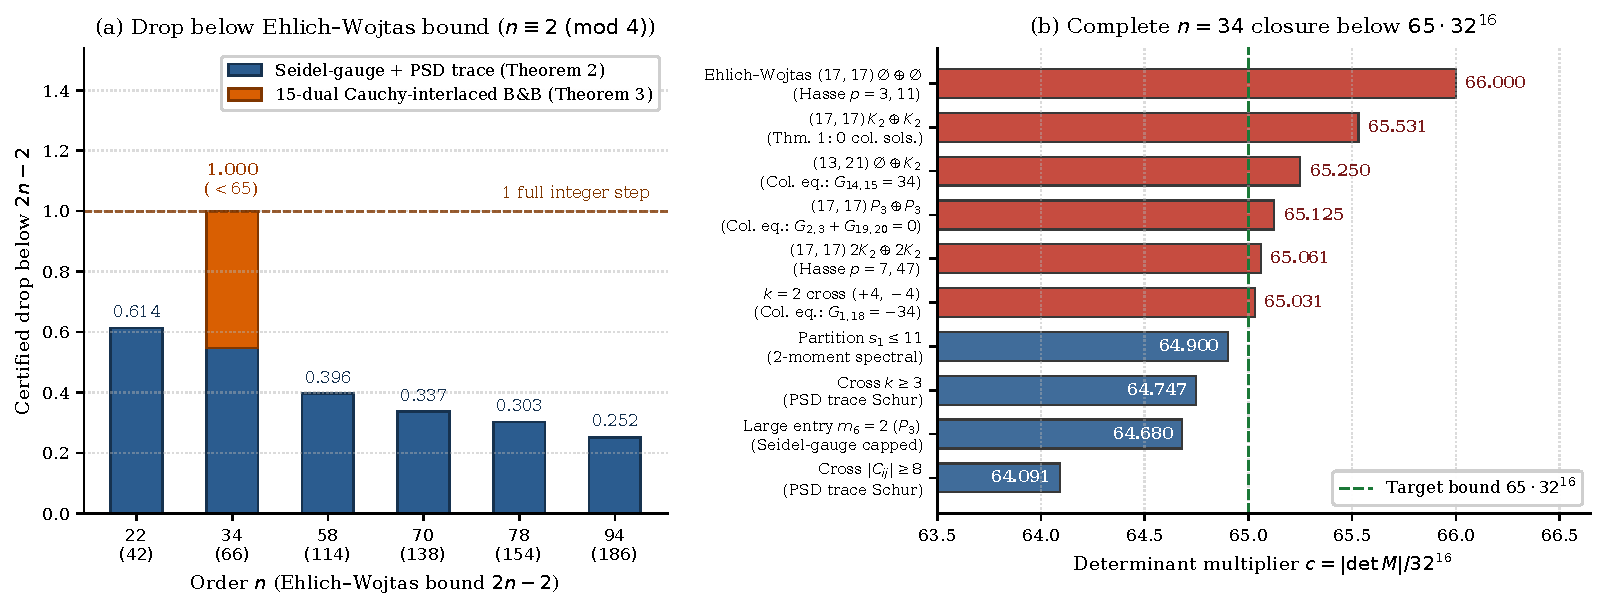
\includegraphics[width=\textwidth]{figures/fig1_r2_unconditional_bounds.pdf}
\caption{Upper bounds for exceptional orders $n \equiv 2 \pmod 4$. (a)~Certified drop below the Ehlich--Wojtas bound $(2n - 2)$ across all exceptional orders $n \le 100$, highlighting the full integer-step drop $66 \to 65$ at $n = 34$ via 15-dual Cauchy-interlaced branch-and-bound. (b)~Complete $n = 34$ closure cascade showing every surviving candidate above $65 \cdot 32^{16}$ (red, all eliminated algebraically) and every remaining spectral or cross-block channel strictly below $65 \cdot 32^{16}$ (blue).}
\label{fig:r2}
\end{figure}

\begin{remark}[Spectral certification and literature context]\label{rem:dedup}
All algebraic eliminations (determinants, Hasse--Minkowski invariants, column equations, and integer Farkas certificates) run in exact arbitrary-precision integer or rational arithmetic. Across all spectral steps of Theorems~\ref{thm:r2_all} and~\ref{thm:d34} (where block dimension satisfies $s \le 51$, since $s_{1,\min}(94) = 43$ implies $s_2 \le 94 - 43 = 51$), every symmetric eigendecomposition $(\hat{\Lambda}, \hat{V})$ of a $k \times k$ integer block $B$ is certified a posteriori via the exact polar-factor Weyl bound: writing $\hat{V} = Q P$ with $Q^\top Q = I$, $P = (\hat{V}^\top \hat{V})^{1/2}$, and $\eta := \|\hat{V}^\top \hat{V} - I\|_F < \frac{1}{2}$, we have $\|Q - \hat{V}\|_2 = \|P - I\|_2 \le \eta / (1 + \sqrt{1 - \eta}) < \eta$, and the identity
\[
  B - Q\hat{\Lambda}Q^\top
  = (B\hat{V} - \hat{V}\hat{\Lambda}) Q^\top + B(Q - \hat{V})Q^\top + (\hat{V} - Q)\hat{\Lambda} Q^\top
\]
yields $\max_i |\lambda_i(B) - \hat{\lambda}_i| \le \|B\hat{V} - \hat{V}\hat{\Lambda}\|_F + (\|B\|_F + \|\hat{\Lambda}\|_2)\,\eta$ by Weyl's inequality. For all spectral nodes of Theorem~\ref{thm:r2_all} ($n \in \{22, 34, 58, 70, 78, 94\}$) and Steps~1 and~4 of Theorem~\ref{thm:d34}, we round LAPACK's floating-point output to an exact dyadic pair $\hat{V} = 2^{-52}\widetilde{V}$, $\hat{\Lambda} = 2^{-45}\widetilde{\Lambda}$ ($\widetilde{V}, \widetilde{\Lambda}$ integer) and evaluate $\|B\hat{V} - \hat{V}\hat{\Lambda}\|_F$, $\|\hat{V}^\top \hat{V} - I\|_F$, and the Davis--Kahan~\cite{daviskahan1970} top-eigenvector bound
\[
  \min_{\sigma = \pm 1}\|v_1 - \sigma u_1\|_\infty
  \le \frac{\sqrt{2}\,\|Bu_1 - \hat{\lambda}_1 u_1\|_2}{\hat{\lambda}_1 - \hat{\lambda}_2 - 2\delta_{\mathrm{Weyl}}}
\]
entirely in exact integer and rational arithmetic, where $v_1$ denotes the true top unit eigenvector of $B$ and $u_1 := \hat{v}_1 / \|\hat{v}_1\|_2$ is the normalized top column of $\hat{V}$ (achieving $\delta_{\mathrm{Weyl}} < 10^{-11}$ on all Theorem~\ref{thm:r2_all} blocks), substituting conservative upper or lower eigenvalue enclosures according to the sign of $1 - a_1 - a_2$. Across the vectorized Step~2 branch-and-bound tree of Theorem~\ref{thm:d34} ($k \le 22$), we bound the IEEE~754 \texttt{float64} evaluation error of $\|B\hat{V} - \hat{V}\hat{\Lambda}\|_F$ and $\|\hat{V}^\top\hat{V} - I\|_F$ analytically via Higham's matrix-product backward-error bound~\cite[\S3.5]{higham2002} ($\gamma_{k+1} = (k+1)u/(1 - (k+1)u)$, $u = 2^{-53}$, achieving $\delta_{\mathrm{Weyl}} < 2 \times 10^{-11}$), explicitly prune non-positive-definite intermediates ($\hat{\beta}_j + \delta_{\mathrm{Weyl}} \le 0$), and evaluate Proposition~\ref{prop:tangent_dual} on the enlarged certified intervals $[\max(10^{-6}, \hat{\beta}_i - \delta_{\mathrm{Weyl}}),\, \hat{\beta}_i + \delta_{\mathrm{Weyl}}]$ with an additional $10^{-6}$ pruning margin. Clamping $l_i$ from $0$ up to $10^{-6}$ is mathematically sound: every tangent pair in Step~2 satisfies $x_1 \ge 28 > 10^{-6}$ and $g$ is strictly increasing on $(0, x_1)$, so any true eigenvalue $\lambda_i \in (0, 10^{-6})$ obeys $g(\lambda_i) < g(10^{-6})$, meaning the clamp can only increase the upper bound~\eqref{eq:tangent_dual}. Post-enclosure scalar evaluations of $\exp$, $\log$, and $\sqrt{\cdot}$ use standard IEEE~754 \texttt{float64} arithmetic verified against positive certification margins: in Theorem~\ref{thm:r2_all}, the minimum absolute margin is $5.78 \times 10^{-5}$ at $n = 34$ ($65.453 - 65.452942 \approx 5.78 \times 10^{-5}$, relative margin $\ge 8.8 \times 10^{-7}$); in Theorem~\ref{thm:d34}, the minimum absolute margin is $> 0.100$ in Step~1 ($65 - 64.8999 = 0.1001$, relative margin $\ge 1.5 \times 10^{-3}$), $10^{-6}$ at pruning nodes in Step~2 ($\theta_s \le \theta_{22} \approx 75.446$, relative margin $\ge 1.3 \times 10^{-8}$), and $> 0.253$ for the Step~4 $|C_{ij}| \ge 8$ and $k \ge 3$ spectral bounds ($65 - 64.7464 > 0.253$, relative margin $\ge 3.9 \times 10^{-3}$) together with a $10^{-6}$ tolerance at the Step~4 $k = 2$ PSD trace pre-filter (relative margin $\ge 1.5 \times 10^{-8}$). Every relative margin therefore exceeds IEEE~754 \texttt{float64} unit roundoff $u = 2^{-53} \approx 1.11 \times 10^{-16}$ by more than eight orders of magnitude ($> 10^8$).

In the $n \equiv 2 \pmod 4$ literature, $n = 22$ was resolved completely ($D(22) = 40 \cdot 20^{10}$) by Chasiotis, Kounias, and Farmakis~\cite{chasiotis2018,chasiotis2019corr} via block-structure case analysis tailored to order $22$; at $n = 34$, where the $2$-moment spectral bound stalls at $65.453 \cdot 32^{16}$, Browne, Egan, Hegarty, and \'O~Cath\'ain~\cite{browne2021survey} catalog $n = 34$ as the smallest open $n \equiv 2 \pmod 4$ order below the Ehlich--Wojtas bound $66 \cdot 32^{16}$~\cite{ehlich1964a,wojtas1964} (with best known constructive lower bounds remaining well below this ceiling~\cite{koukouvinos2000,orrick2003,brent2012maxdet,brent2013lower,browne2021survey}). Theorem~\ref{thm:d34} lowers this upper bound by a full integer multiple of $32^{16}$.
\end{remark}

\section{Exact Algebraic Closures at \texorpdfstring{$n = 29$ and $n = 33$}{n = 29 and n = 33}}\label{sec:r1}

We now apply the four-stage algebraic framework of Section~\ref{sec:algebraic} to the two smallest open orders in the $n \equiv 1 \pmod 4$ class. For $n = 29$, a \emph{Gram-class signature} $(c_1, c_3, c_5)$ counts unordered off-diagonal pairs $\{i, j\}$ ($1 \le i < j \le 29$, $c_1 + c_3 + c_5 = \binom{29}{2} = 406$) with $|G_{ij}| = 1, 3, 5$ respectively, so $\tr(G^2) = 29^3 + 2(c_1 + 9c_3 + 25c_5)$. Normalizing row~$1$ of $M$ to $(+1)^{29}$ (by column negations) and orienting rows $2, \dots, 29$ (by row negations) yields non-negative row sums $r_i = G_{1i} \in \{1, 3, 5\}$ for $i \in \{2, \dots, 29\}$. Let $p_3$ and $p_5$ count the rows $i \ge 2$ with $r_i = 3$ and $r_i = 5$ respectively, leaving $28 - p_3 - p_5$ rows with $r_i = 1$, and leaving $c_3 - p_3$ outside pairs of magnitude $3$ and $c_5 - p_5$ outside pairs of magnitude $5$ among $\{2, \dots, 29\}$. We define a \emph{canonical spread placement} for $(c_1, c_3, c_5)$ and $(p_3, p_5)$ to be the assignment placing all $(c_3 - p_3)$ outside magnitude-$3$ pairs and all $(c_5 - p_5)$ outside magnitude-$5$ pairs as mutually vertex-disjoint pairs entirely within the $28 - p_3 - p_5$ vertices having $r_i = 1$. Such a placement exists if and only if
\[
  p_3 + p_5 + 2\bigl((c_3 - p_3) + (c_5 - p_5)\bigr) \le 28,
\]
so a signature admits at least one canonical spread placement if and only if $c_3 + c_5 \le 28$. Because all $28 - p_3 - p_5$ vertices with $r_i = 1$ are symmetric relative to row~$1$ and the $r_i \in \{3, 5\}$ rows, and~\eqref{eq:div4} uniquely forces the sign of every odd off-diagonal entry $G_{ij}$ from $(r_i, r_j, |G_{ij}|)$, a canonical spread placement determines the signed Gram matrix $G$ uniquely up to simultaneous row and column permutation. In their unpublished preprint, Brent, Orrick, Osborn, and Zimmermann~\cite{brent2012maximal} report $320 \cdot 7^{12} \cdot 2^{28} \le D(29) < 329 \cdot 7^{12} \cdot 2^{28}$ and note that if $7^{13}$ divides $D(29)/2^{28}$ then $D(29) = 322 \cdot 7^{12} \cdot 2^{28}$; Solomon's $320 \cdot 7^{12} \cdot 2^{28}$ realization has Gram-class signature $(393, 4, 9)$ at $\tr(G^2) = 25697$.

\begin{figure}[ht]
\centering
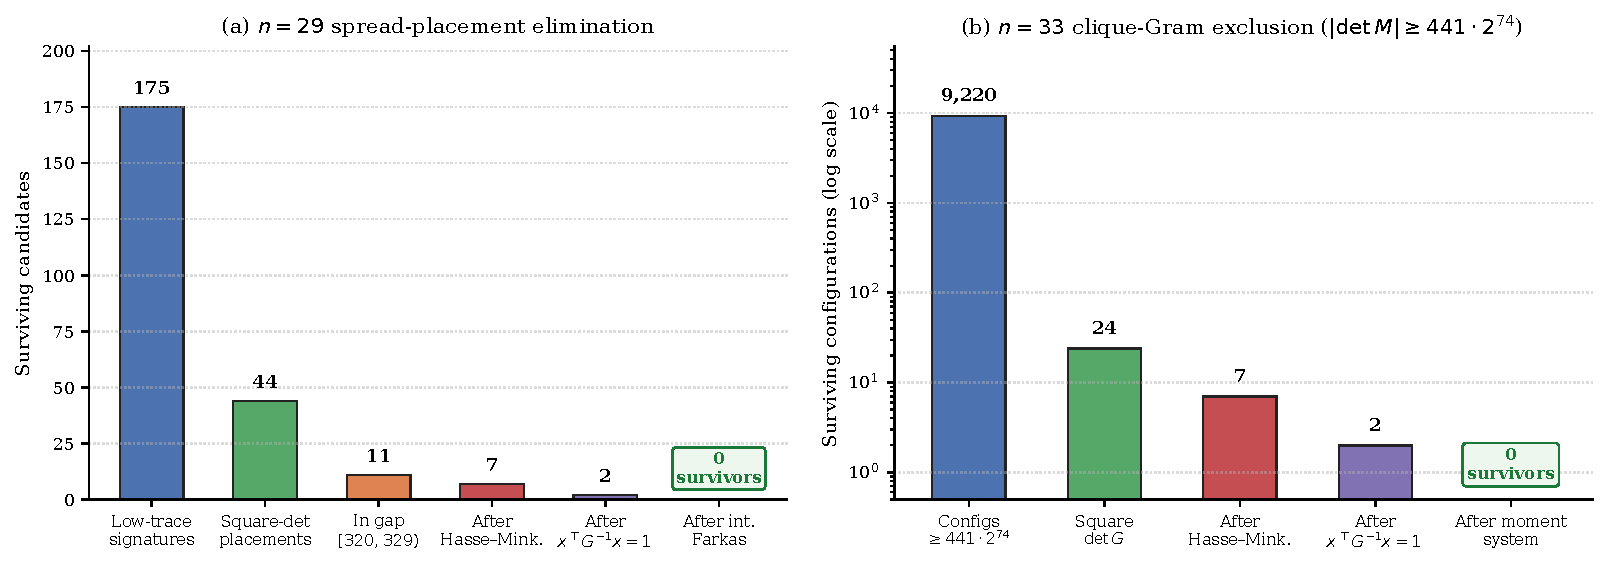
\includegraphics[width=\textwidth]{figures/fig2_algebraic_feasibility_cascade.pdf}
\caption{Exact algebraic elimination cascades in the $n \equiv 1 \pmod 4$ class. (a)~At $n = 29$, $175$ low-trace signatures reduce to $11$ open spread-placement candidates in $[320, 329) \cdot 7^{12} \cdot 2^{28}$, all $11$ of which are eliminated in exact arithmetic. (b)~At $n = 33$, the $9{,}220$ complete $G - J_{33} \succ 0$ clique configurations with $G - J_{33}$ block-diagonal (off-diagonal entries in $\{-7, -3, 1, 5, 9\}$) and $|\det M| \ge 441 \cdot 2^{74}$ (enumerated across $659{,}380$ visited search-tree nodes in exact integer branch-and-bound) collapse through exact algebraic filters to $0$ realizable survivors.}
\label{fig:r1}
\end{figure}

\begin{theorem}[Algebraic closures at $n = 29$ and $n = 33$]\label{thm:r1_close}
\leavevmode
\begin{enumerate}[leftmargin=*,topsep=2pt,itemsep=1pt]
\item \emph{(Order $n = 29$.)} Among all $175$ non-Barba ($c_3 + c_5 \ge 1$) $\{1, 3, 5\}$-supported Gram-class signatures $(c_1, c_3, c_5)$ with $\tr(G^2) < 25697$, $2$ admit no canonical spread placement ($(377, 29, 0)$ and $(376, 30, 0)$), $139$ have no canonical spread placement with perfect-square $\det G$, and the remaining $34$ yield exactly $44$ perfect-square canonical spread placements, partitioned by determinant magnitude into $26$ with $|\det M| \ge 329 \cdot 7^{12} \cdot 2^{28}$, $7$ with $|\det M| < 320 \cdot 7^{12} \cdot 2^{28}$, and $11$ with $|\det M| \in [320, 329) \cdot 7^{12} \cdot 2^{28}$. None of the $11$ placements in $[320, 329) \cdot 7^{12} \cdot 2^{28}$ is realizable as $M M^\top$ for $M \in \{\pm 1\}^{29 \times 29}$ (Table~\ref{tab:h29close}).
\item \emph{(Order $n = 33$.)} No Gram matrix $G = 32 I_{33} + J_{33} + 4 E$ whose shifted matrix $G - J_{33} = 32 I_{33} + 4 E$ is block-diagonal---where $E$ is a disjoint union of uniform-weight cliques $(s_i, w_i)$ with $w_i \in \{-2, -1, +1, +2\}$ and isolated vertices (so off-diagonal entries of $G$ lie in $\{-7, -3, 1, 5, 9\}$)---and satisfying $|\det M| \ge 441 \cdot 2^{74}$ (Solomon's lower bound) is realizable as $M M^\top$ for $M \in \{\pm 1\}^{33 \times 33}$.
\end{enumerate}
\end{theorem}

\begin{proof}
For $n = 29$, exact Bareiss integer determinants over all valid canonical spread placements of the $175$ low-trace signatures reduce the enumeration to the $11$ candidates in $[320, 329) \cdot 7^{12} \cdot 2^{28}$ listed in Table~\ref{tab:h29close}. Applying Section~\ref{sec:algebraic}: four fail Hasse--Minkowski with $c_2(G) = c_3(G) = -1$; two have zero solutions to~\eqref{eq:colnorm}; three force identical rows on outside special pairs ($|G_{ij}| = 29$); and both candidates at $322 \cdot 7^{12} \cdot 2^{28}$ are eliminated by explicit integer Farkas certificates~\eqref{eq:farkas}. Indexing the $10$ moment coordinates by $(1, s_3, s_5, s_1, s_3^2, s_5^2, s_1^2, s_3 s_5, s_3 s_1, s_5 s_1)$, where $s_3, s_5, s_1$ denote the column sums over the row-sum orbits of values $3, 5, 1$ respectively:
\begin{itemize}[leftmargin=*,topsep=1pt,itemsep=1pt]
\item For $(389, 14, 3)$ at $(p_3, p_5) = (14, 3)$ (orbit sizes $14, 3, 11$ and $20$ allowed column types), the integer vector $y = (-18, 0, -1, -3, 1, 0, 0, 1, 0, 0)$ satisfies
\[
  s_3^2 + s_3 s_5 - s_5 - 3 s_1 - 18 \ge 0
\]
on every allowed column type, whereas summing over all $29$ columns of $M$ must equal $588 + (-42) - 15 - 3(11) - 18(29) = -24 < 0$.
\item For $(393, 8, 5)$ at $(p_3, p_5) = (8, 5)$ (orbit sizes $8, 5, 15$ and $45$ allowed column types), the integer vector $y = (0, 0, 0, 7, 0, 0, -1, 0, 0, -2)$ satisfies
\[
  7 s_1 - s_1^2 - 2 s_5 s_1 \ge 0
\]
on every allowed column type, whereas summing over all $29$ columns must equal $7(15) - 645 - 2(75) = -690 < 0$.
\end{itemize}
Note that the final entry $(393, 7, 6)$ at $(6, 6)$ attains $\sqrt{\det G} = 320 \cdot 7^{12} \cdot 2^{28}$ yet is unrealizable; there is no contradiction with the lower bound $D(29) \ge 320 \cdot 7^{12} \cdot 2^{28}$ because Solomon's $320 \cdot 7^{12} \cdot 2^{28}$ matrix realizes a different Gram signature, namely $(393, 4, 9)$.

For $n = 33$, writing $G = 4 A + J$ with $A = 8 I + E$ gives $\det G = 4^{32} \det(A)\bigl(4 + \mathbf{1}^\top A^{-1}\mathbf{1}\bigr)$ whenever $A$ is invertible. Since $G$ is a rank-$1$ positive update of $4A$, positive-definiteness of $G$ allows at most one block $(s, w)$ of $A$ to have its simple eigenvalue $\lambda_1 = 8 + (s - 1)w \le 0$. Any configuration containing a $\lambda_1 = 0$ block ($(9, -1)$ or $(5, -2)$) satisfies $\det G = 4^{32} s (8 - w)^{s-1} \det(A_{\mathrm{rest}}) \le 4^{32} s (8 - w)^{s-1} 8^{33-s}$, giving $|\det M| = \sqrt{\det G} \le 307.55 \cdot 2^{74}$ for $(9, -1)$ and $|\det M| = \sqrt{\det G} \le 223.61 \cdot 2^{74}$ for $(5, -2)$, both strictly below $441 \cdot 2^{74}$. Likewise, any configuration with one $\lambda_1 < 0$ block ($s \ge 10, w = -1$ or $s \ge 6, w = -2$) satisfies $\det G = 4^{32} |\lambda_1| (8 - w)^{s-1} \det(A_{\mathrm{rest}}) \bigl(\frac{s}{|\lambda_1|} - 4 - \mathbf{1}^\top A_{\mathrm{rest}}^{-1}\mathbf{1}\bigr) < 4^{32}(8 - w)^{s-1}(s - 4|\lambda_1|) 8^{33-s}$. Because $G \succ 0$ requires $\det G > 0$, this forces $s - 4|\lambda_1| > 0$, immediately eliminating all $s \ge 12$ ($w = -1$, where $s - 4|\lambda_1| = 36 - 3s \le 0$) and all $s \ge 6$ ($w = -2$, where $s - 4|\lambda_1| = 40 - 7s < 0$) and leaving only $(s, w) \in \{(10, -1), (11, -1)\}$, for which the positive upper bound yields $|\det M| = \sqrt{\det G} < 267 \cdot 2^{74} < 441 \cdot 2^{74}$. Thus every configuration attaining $|\det M| \ge 441 \cdot 2^{74}$ has $A \succ 0$ ($\lambda_1 > 0$ on every block).

An exact branch-and-bound depth-first search over all $A \succ 0$ clique configurations, using $\det(B_i) \le 8^{s_i}$ (by AM--GM) and the maximum per-vertex increment $\max_{(s, w)} (\lambda_1^{-1} - 8^{-1})$ scaled by the common denominator $\operatorname{lcm}(8, \{\lambda_1\})$ so that every determinant and pruning test executes entirely in exact integer arithmetic, visits $659{,}380$ search-tree nodes ($54{,}991$ for $w_i \in \{\pm 1\}$) and exhaustively enumerates all $9{,}220$ complete $A \succ 0$ clique-multiset configurations attaining $|\det M| \ge 441 \cdot 2^{74}$ ($3{,}764$ for $w_i \in \{\pm 1\}$). Exactly $24$ have perfect-square determinant: $17$ fail Hasse--Minkowski, $3$ have zero solutions to~\eqref{eq:colnorm}, $2$ force identical or opposite rows, and the final $2$ have elementary exact column-moment obstructions (Figure~\ref{fig:r1}b). For both remaining Gram matrices, we partition the $33$ rows into three block families $A$, $B$, $C$ (where $A$ consists of $(2, -1)$ blocks, $B$ of $(2, +1)$ blocks, and $C$ of a single $3$-block). For any column $x \in \{\pm 1\}^{33}$, let $s_a := \sum_{i \in a} x_i \in \{-2, 0, 2\}$ for each $2$-block $a \in A$, let $n_{A,2} := |\{a \in A : |s_a| = 2\}|$ (so $\sum_{a \in A} s_a^2 = 4 n_{A,2}$), define $s_b$ and $n_{B,2}$ analogously for $b \in B$, and set aggregate sums $s_A := \sum_{i \in A} x_i$, $s_B := \sum_{i \in B} x_i$, and $s_C := \sum_{i \in C} x_i \in \{-3, -1, 1, 3\}$:
\begin{itemize}[leftmargin=*,topsep=1pt,itemsep=1pt]
\item $13\cdot(2,-1) + 2\cdot(2,+1) + 1\cdot(3,+1)$ ($A$ has $13$ blocks, $B$ has $2$ blocks, $C = (3, +1)$): exact solution of~\eqref{eq:colnorm} yields $3$ allowed triples $(n_{A,2}, n_{B,2}, s_C^2) \in \{(4,0,1), (6,2,1), (9,1,9)\}$ with column counts $n_0, n_1, n_2 \in \Z_{\ge 0}$. The total-count equation $n_0 + n_1 + n_2 = 33$, the $C$-block moment $\sum_{\mathrm{cols}} s_C^2 = 3 \cdot 33 + 6 \cdot 5 = 129 \implies 33 + 8 n_2 = 129 \implies n_2 = 12$, and the per-block $B$-moment $\sum_{\mathrm{cols}} \sum_{b \in B} s_b^2 = 2(2 \cdot 33 + 2 \cdot 5) = 152 \implies 2 n_1 + n_2 = 38$ uniquely force $(n_0, n_1, n_2) = (8, 13, 12)$. This contradicts the per-block $A$-moment $\sum_{\mathrm{cols}} \sum_{a \in A} s_a^2 = 13(2 \cdot 33 - 2 \cdot 3) = 780$, which requires $4 n_0 + 6 n_1 + 9 n_2 = 195$, whereas $4(8) + 6(13) + 9(12) = 218 \ne 195$.
\item $12\cdot(2,-1) + 3\cdot(2,+1) + 1\cdot(3,-1)$ ($A$ has $12$ blocks, $B$ has $3$ blocks, $C = (3, -1)$): exact solution of~\eqref{eq:colnorm} yields $9$ allowed tuples $(n_{A,2}, n_{B,2}, s_C^2, s_A s_B)$, of which only $(3, 3, 9, +12)$ has positive cross-moment $s_A s_B > 0$ (all other $8$ satisfy $s_A s_B \le 0$). Thus $\sum_{\mathrm{cols}} s_A s_B = \mathbf{1}_A^\top G \mathbf{1}_B = 24 \cdot 6 = 144$ forces at least $144/12 = 12$ columns with $s_C^2 = 9$, contradicting $\sum_{\mathrm{cols}} s_C^2 = 3 \cdot 33 + 6(-3) = 81$, which allows only $(81 - 33)/8 = 6$ such columns.\qedhere
\end{itemize}
\end{proof}

In the context of the $n = 29$ literature, the $7$ perfect-square spread placements below $320 \cdot 7^{12} \cdot 2^{28}$ fall beneath Solomon's constructive lower bound~\cite{orrick2003,brent2012maxdet}, while the $26$ placements with $|\det M| \ge 329 \cdot 7^{12} \cdot 2^{28}$ lie at or above the ceiling $329 \cdot 7^{12} \cdot 2^{28}$ (where the unpublished preprint of Brent, Orrick, Osborn, and Zimmermann~\cite{brent2012maximal} reports the strict upper bound $D(29) < 329 \cdot 7^{12} \cdot 2^{28}$); Theorem~\ref{thm:r1_close}(1) itself is unconditional and establishes the exact determinant partition together with algebraic non-realizability of all $11$ placements in $[320, 329) \cdot 7^{12} \cdot 2^{28}$.

\begin{table}[ht]
\centering
\caption{Exact elimination of all $11$ residual $n = 29$ canonical spread-placement candidates in $[320, 329) \cdot 7^{12} \cdot 2^{28}$.}
\label{tab:h29close}
\small
\begin{tabular}{llrl}
\toprule
\textbf{Signature} & $(p_3, p_5)$ & $|\det M| / (7^{12} 2^{28})$ & \textbf{Exact elimination mechanism} \\
\midrule
$(394, 6, 6)$  & $(0, 2)$  & 328.343 & Hasse--Minkowski ($c_2 = c_3 = -1$) \\
$(389, 13, 4)$ & $(12, 0)$ & 326.264 & Column eq.~\eqref{eq:colnorm}: $3$ types, all force identical $-3/+5$ pairs \\
$(389, 12, 5)$ & $(12, 1)$ & 322.426 & Column eq.~\eqref{eq:colnorm}: $4$ types, all force identical $+5$ pairs \\
$(394, 4, 8)$  & $(4, 4)$  & 322.426 & Column eq.~\eqref{eq:colnorm}: $0$ solutions \\
$(391, 11, 4)$ & $(3, 4)$  & 322.291 & Column eq.~\eqref{eq:colnorm}: $0$ solutions \\
$(393, 7, 6)$  & $(7, 4)$  & 322.286 & Hasse--Minkowski ($c_2 = c_3 = -1$) \\
$(391, 10, 5)$ & $(1, 4)$  & 322.028 & Hasse--Minkowski ($c_2 = c_3 = -1$) \\
$(389, 14, 3)$ & $(14, 3)$ & \textbf{322.000} & Exact Farkas: $s_3^2 + s_3 s_5 - s_5 - 3s_1 - 18 \ge 0$ vs.\ $-24 < 0$ \\
$(393, 8, 5)$  & $(8, 5)$  & \textbf{322.000} & Exact Farkas: $7 s_1 - s_1^2 - 2 s_5 s_1 \ge 0$ vs.\ $-690 < 0$ \\
$(392, 6, 8)$  & $(0, 5)$  & 320.450 & Hasse--Minkowski ($c_2 = c_3 = -1$) \\
$(393, 7, 6)$  & $(6, 6)$  & 320.000 & Column eq.~\eqref{eq:colnorm}: $11$ types, all force identical $-3$ pairs \\
\bottomrule
\end{tabular}
\end{table}

\section{Concluding Remarks}\label{sec:concluding}

The results of Sections~\ref{sec:k2k2}--\ref{sec:r1} point directly to three natural open problems. First, at $n = 34$, Theorem~\ref{thm:d34} lowers the upper bound from $66 \cdot 32^{16}$ to $65 \cdot 32^{16}$, yet a substantial gap remains to the best known constructive lower bounds~\cite{orrick2003,browne2021survey}; pushing the Cauchy-interlaced Lagrange-dual branch-and-bound below $64 \cdot 32^{16}$ will require tighter switching-class canonicalization and sharper multi-entry cross-block bounds for $k \in \{3, 4\}$. Second, extending the same branch-and-bound framework to the next exceptional order $n = 58$ (where Theorem~\ref{thm:r2_all} gives $D(58) < 113.604 \cdot 56^{28}$ against the Ehlich--Wojtas ceiling $114 \cdot 56^{28}$) could establish a full integer-step improvement $D(58) < 113 \cdot 56^{28}$ if larger principal submatrix sizes can be pruned efficiently. Third, Theorem~\ref{thm:r1_close} does not settle $D(29)$ or $D(33)$ unconditionally: lifting the structural restrictions requires handling overlapping (non-spread) special-pair placements and signatures with $\tr(G^2) \ge 25697$ at $n = 29$, and non-clique off-diagonal graphs or entries with $|G_{ij}| \ge 11$ at $n = 33$.

\section*{Declarations}

\paragraph{Funding.} This research received no external funding.

\paragraph{Competing Interests.} The author declares no competing interests.

\paragraph{Use of AI-Assisted Tools.} Large language models (Anthropic Claude and Google Gemini) were used during computational exploration, proof drafting, software development, and manuscript editing. All mathematical arguments, exact algebraic eliminations, spectral enclosures, and verification scripts were reviewed, checked, and executed by the author. All figures were generated programmatically from verified computational outputs; no generative AI imagery was used. The author assumes full responsibility for all content.

\paragraph{Data and Code Availability.} All exact-arithmetic verification routines, unit tests, executable proof scripts, figure-generation code, and archived verification logs (in \path{docs/verification_logs/}) are publicly available at \url{https://github.com/Brsanch/hadamard-maxdet}, tagged release \texttt{v1.0.0} at \url{https://github.com/Brsanch/hadamard-maxdet/releases/tag/v1.0.0}. Theorems~\ref{thm:k2k2} and~\ref{thm:r2_all} are verified in \path{tests/test_feasibility.py}, Theorem~\ref{thm:d34} in \path{scripts/prove_h34_below_65.py}, Theorem~\ref{thm:r1_close} in \path{scripts/verify_r1_closures.py}, and Figures~\ref{fig:r2} and~\ref{fig:r1} via \path{paper/scripts/make_hadamard_figures.py}.

\begin{thebibliography}{24}
\setlength{\itemsep}{3pt plus 1pt}

\bibitem{barba1933}
G.~Barba.
Intorno al teorema di Hadamard sui determinanti a valore massimo.
\emph{Giorn.\ Mat.\ Battaglini}, 71:70--86, 1933.

\bibitem{brent2012maxdet}
R.~P.~Brent.
The Hadamard maximal determinant problem.
Online resource, \url{https://maths-people.anu.edu.au/~brent/maxdet/}.

\bibitem{brent2012maximal}
R.~P.~Brent, W.~P.~Orrick, J.-A.~H.~Osborn, and P.~Zimmermann.
Maximal determinants and saturated $D$-optimal designs of orders $19$ and $37$.
Preprint, arXiv:1112.4160, 2012.

\bibitem{brent2013lower}
R.~P.~Brent and J.-A.~H.~Osborn.
General lower bounds on maximal determinants of binary matrices.
\emph{Electron.\ J.\ Combin.}, 20(2):\#P15, 2013.

\bibitem{brouwer2012}
A.~E.~Brouwer and W.~H.~Haemers.
\emph{Spectra of Graphs}.
Universitext, Springer, New York, 2012.

\bibitem{browne2021survey}
P.~Browne, R.~Egan, F.~Hegarty, and P.~\'O~Cath\'ain.
A survey of the Hadamard maximal determinant problem.
\emph{Electron.\ J.\ Combin.}, 28(4):\#P4.41, 2021.

\bibitem{chadjipantelis1987}
T.~Chadjipantelis, S.~Kounias, and C.~Moyssiadis.
The maximum determinant of $21 \times 21$ $(+1, -1)$-matrices and $D$-optimal designs.
\emph{J.\ Statist.\ Plann.\ Inference}, 16:167--178, 1987.

\bibitem{chasiotis2018}
V.~Chasiotis, S.~Kounias, and N.~Farmakis.
The $D$-optimal saturated designs of order $22$.
\emph{Discrete Math.}, 341(2):380--387, 2018.

\bibitem{chasiotis2019corr}
V.~Chasiotis, S.~Kounias, and N.~Farmakis.
Corrigendum to ``The $D$-optimal saturated designs of order $22$''.
\emph{Discrete Math.}, 342(7):2161, 2019.

\bibitem{cohn1963}
J.~H.~E.~Cohn.
On the value of determinants.
\emph{Proc.\ Amer.\ Math.\ Soc.}, 14(4):581--588, 1963.

\bibitem{daviskahan1970}
C.~Davis and W.~M.~Kahan.
The rotation of eigenvectors by a perturbation.~III.
\emph{SIAM J.\ Numer.\ Anal.}, 7(1):1--46, 1970.

\bibitem{ehlich1964a}
H.~Ehlich.
Determinantenabsch\"atzungen f\"ur bin\"are Matrizen.
\emph{Math.\ Z.}, 83:123--132, 1964.

\bibitem{ehlich1964b}
H.~Ehlich.
Determinantenabsch\"atzungen f\"ur bin\"are Matrizen mit $N \equiv 3 \bmod 4$.
\emph{Math.\ Z.}, 84:438--447, 1964.

\bibitem{farmakis1987}
N.~Farmakis and S.~Kounias.
The excess of Hadamard matrices and optimal designs.
\emph{Discrete Math.}, 67(2):165--176, 1987.

\bibitem{hadamard1893}
J.~Hadamard.
R\'esolution d'une question relative aux d\'eterminants.
\emph{Bull.\ Sci.\ Math.}, 17:240--246, 1893.

\bibitem{higham2002}
N.~J.~Higham.
\emph{Accuracy and Stability of Numerical Algorithms}.
2nd ed., SIAM, Philadelphia, 2002.

\bibitem{koukouvinos2000}
C.~Koukouvinos, M.~Mitrouli, and J.~Seberry.
Bounds on the maximum determinant for $(1, -1)$ matrices.
\emph{Bull.\ Inst.\ Combin.\ Appl.}, 29:39--48, 2000.

\bibitem{moyssiadis1982}
C.~Moyssiadis and S.~Kounias.
The exact $D$-optimal first order saturated design with $17$ observations.
\emph{J.\ Statist.\ Plann.\ Inference}, 7(1):13--27, 1982.

\bibitem{neubauer1997}
M.~G.~Neubauer and A.~J.~Radcliffe.
The maximum determinant of $\pm 1$ matrices.
\emph{Linear Algebra Appl.}, 257:289--306, 1997.

\bibitem{orrick2005}
W.~P.~Orrick.
The maximal $\{-1, 1\}$-determinant of order $15$.
\emph{Metrika}, 62(2):195--219, 2005.

\bibitem{orrick2003}
W.~P.~Orrick, B.~Solomon, R.~Dowdeswell, and W.~D.~Smith.
New lower bounds for the maximal determinant problem.
Preprint, arXiv:math/0304410, 2003.

\bibitem{orrick2007}
W.~P.~Orrick and B.~Solomon.
Large-determinant sign matrices of order $4k+1$.
\emph{Discrete Math.}, 307(2):226--236, 2007.

\bibitem{serre1973}
J.-P.~Serre.
\emph{A Course in Arithmetic}.
Graduate Texts in Mathematics, vol.~7, Springer, New York, 1973.

\bibitem{wojtas1964}
M.~Wojtas.
On Hadamard's inequality for the determinants of order non-divisible by $4$.
\emph{Colloq.\ Math.}, 12:73--83, 1964.

\end{thebibliography}

\end{document}
